
\documentclass[11pt]{iopart}
%DIF 3a3
\usepackage[pdftex,bookmarks,pagebackref]{hyperref} %DIF > 
%DIF -------

\usepackage{epsfig}
\usepackage{color}

\usepackage{amssymb}
\usepackage{amsfonts}
\usepackage{graphicx}
\usepackage{iopams}
\graphicspath{figures/}
\usepackage{lineno}

%DIF 14c15
%DIF < \newcommand{\jvnote}[1]{{\color{green}[#1]}}
%DIF -------
\newcommand{\dsnote}[1]{{\color{green}[#1]}} %DIF > 
%DIF -------

%%%%%%%%%%%%%%%%%%%%%%%%%%%%%%%%%%%%%%%%%%%%%%%%%%%%%%%%%%%%%%%%%%%%%%%%%%%%%%%%%%%%%%
%DIF PREAMBLE EXTENSION ADDED BY LATEXDIFF
%DIF UNDERLINE PREAMBLE %DIF PREAMBLE
\RequirePackage[normalem]{ulem} %DIF PREAMBLE
\RequirePackage{color}\definecolor{RED}{rgb}{1,0,0}\definecolor{BLUE}{rgb}{0,0,1} %DIF PREAMBLE
\providecommand{\DIFaddtex}[1]{{\protect\color{blue}\uwave{#1}}} %DIF PREAMBLE
\providecommand{\DIFdeltex}[1]{{\protect\color{red}\sout{#1}}}                      %DIF PREAMBLE
%DIF SAFE PREAMBLE %DIF PREAMBLE
\providecommand{\DIFaddbegin}{} %DIF PREAMBLE
\providecommand{\DIFaddend}{} %DIF PREAMBLE
\providecommand{\DIFdelbegin}{} %DIF PREAMBLE
\providecommand{\DIFdelend}{} %DIF PREAMBLE
%DIF FLOATSAFE PREAMBLE %DIF PREAMBLE
\providecommand{\DIFaddFL}[1]{\DIFadd{#1}} %DIF PREAMBLE
\providecommand{\DIFdelFL}[1]{\DIFdel{#1}} %DIF PREAMBLE
\providecommand{\DIFaddbeginFL}{} %DIF PREAMBLE
\providecommand{\DIFaddendFL}{} %DIF PREAMBLE
\providecommand{\DIFdelbeginFL}{} %DIF PREAMBLE
\providecommand{\DIFdelendFL}{} %DIF PREAMBLE
%DIF END PREAMBLE EXTENSION ADDED BY LATEXDIFF
%DIF PREAMBLE EXTENSION ADDED BY LATEXDIFF
%DIF HYPERREF PREAMBLE %DIF PREAMBLE
\providecommand{\DIFadd}[1]{\texorpdfstring{\DIFaddtex{#1}}{#1}} %DIF PREAMBLE
\providecommand{\DIFdel}[1]{\texorpdfstring{\DIFdeltex{#1}}{}} %DIF PREAMBLE
%DIF END PREAMBLE EXTENSION ADDED BY LATEXDIFF

\begin{document}

\title[Gate Hadron PET]{Feasibility \DIFdelbegin \DIFdel{of a Monte Carlo full-scaled }\DIFdelend \DIFaddbegin \DIFadd{study for GATE }\DIFaddend simulation of
  \DIFdelbegin \DIFdel{patient }\DIFdelend \DIFaddbegin \DIFadd{hadrontherapy }\DIFaddend dose deposition combined with \DIFaddbegin \DIFadd{a complete }\DIFaddend PET imaging
  \DIFdelbegin \DIFdel{during pencil beam spot scanning with $^{12}$C ion beams using GATE on a HPC cluster}\DIFdelend \DIFaddbegin \DIFadd{system.}\DIFaddend }

%DIF > Feasibility of a Monte Carlo full-scaled
%DIF >   simulation of patient dose deposition combined with PET imaging
%DIF >   during pencil beam spot scanning with $^{12}$C ion beams using GATE
%DIF >   on a HPC cluster}
\DIFaddbegin 

\DIFaddend \author{S{\'e}bastien Jan$^{1}$, Thibault Frisson$^{2,3}$, and David Sarrut $^{2,3}$}

\address{$^1$ CEA, Service Hospitalier Frédéric Joliot, Orsay, France}
\address{$^2$ University of Lyon, CREATIS-LRMN; CNRS UMR5220; INSA-Lyon, France}
\address{$^3$ University of Lyon, L\'eon B\'erard Cancer Center, F-69373, Lyon, France}
\ead{david.sarrut@creatis.insa-lyon.fr}

%%%%%%%%%%%%%%%%%%%%%%%%%%%%%%%%%%%%%%%%%%%%%%%%%%%%%%%%%%%%%%%%%%%%%%%%%%%%%%%%%%%%%%
\linenumbers
\begin{abstract}\\

  {\it \DIFdelbegin \DIFdel{Objectives}\DIFdelend \DIFaddbegin \DIFadd{Objective}\DIFaddend \\
    \DIFdelbegin \DIFdel{The goal of this paper is to report a feasibility to perform }\DIFdelend \DIFaddbegin \DIFadd{We report the feasibility study of performing }\DIFaddend with GATE a
    full-scaled simulation of the patient dose deposition combined
    with complete PET imaging\DIFdelbegin \DIFdel{obtained from }\DIFdelend \DIFaddbegin \DIFadd{. Dose distribution and PET image are
    obtained from a carbon ion irradiation using }\DIFaddend pencil beam spot
    scanning \DIFdelbegin \DIFdel{with carbon ion in hadrontherapy}\DIFdelend \DIFaddbegin \DIFadd{delivery}\DIFaddend . This study shows the possibility to \DIFdelbegin \DIFdel{simulated a complex treatment delivery together with full PET imaging to control the dose and
    scale on }\DIFdelend \DIFaddbegin \DIFadd{simulate
    with the same Monte-Carlo platform such complex treatment and
    imaging processes. We also show that it scales well on a }\DIFaddend large
    number of CPUs.
  }\\

  {\it Methods\\
    Using the GATE \DIFdelbegin \DIFdel{plateform; Explicit }\DIFdelend \DIFaddbegin \DIFadd{platform; explicit }\DIFaddend simulation from the beam to the
    patient and from the patient to the PET scanner system. \DIFaddbegin \DIFadd{Scaling
    was assessed on a 1000 CPUs cluster.
  }\DIFaddend }\\

  {\it Results\\
    First full-scale simulation in the \DIFdelbegin \DIFdel{way }\DIFdelend \DIFaddbegin \DIFadd{context }\DIFaddend of hadrontherapy
    including dose monitoring with PET imaging. The dose monitoring
    for $^{12}$C irradiation should be realistic and feasible for a
    target dose higher than 1 Gy.
  }\\

  {\it Conclusions\\
    GATE is adapted to perform \DIFdelbegin \DIFdel{very high realistic simulation }\DIFdelend \DIFaddbegin \DIFadd{highly realistic simulations }\DIFaddend in the
    field of hadrontherapy\DIFaddbegin \DIFadd{, combining dose }\DIFaddend and imaging system to
    \DIFdelbegin \DIFdel{control }\DIFdelend \DIFaddbegin \DIFadd{monitor }\DIFaddend the dose delivery during a \DIFdelbegin \DIFdel{radiation planning}\DIFdelend \DIFaddbegin \DIFadd{cancer treatment}\DIFaddend . This approach
    should be use to develop and optimize imaging systems for
    hadrontherapy applications \DIFdelbegin \DIFdel{ans also to define protocols where an imaging control will be feasible for a quantitative analysis}\DIFdelend \DIFaddbegin \DIFadd{and to determine the feasibility of
    quantitative imaging protocols}\DIFaddend .
  }\\

\end{abstract}

%Uncomment for PACS numbers title message
%\pacs{00.00, 20.00, 42.10}
% Keywords required only for MST, PB, PMB, PM, JOA, JOB? 
\vspace{2pc}
\noindent{\it Keywords}: Monte Carlo ; GATE ; Hadrontherapy ; PET monitoring
% Uncomment for Submitted to journal title message
%\submitto{\PMB}
% Comment out if separate title page not required
\maketitle


%%%%%%%%%%%%%%%%%%%%%%%%%%%%%%%%%%%%%%%%%%%%%%%%%%%%%%%%%%%%%%%%%%%%%%%%%%%%%%%%%%%%%%%
\section{Introduction}
\DIFaddbegin 

\DIFaddend Monte Carlo simulations are essential for many medical applications,
especially for imaging and radiotherapy. Numerical approaches for
imaging applications are used to design new devices, to optimize and
study the effect of acquisition parameters on the image quality. They
are also extremely useful to validate and assess compensation methods
and image reconstruction techniques. \DIFdelbegin \DIFdel{For radiotherapy applications}\DIFdelend \DIFaddbegin \DIFadd{In the radiation therapy field}\DIFaddend ,
Monte Carlo simulations are used to develop \DIFdelbegin \DIFdel{planning treatments so as to optimize the dose distribution in tumour and organs at risk. In this research context, the GATE~}%DIFDELCMD < \cite{Jan2004,Jan2011} %%%
\DIFdel{simulation platform}\DIFdelend \DIFaddbegin \DIFadd{fast dose deposition
algorithms or to characterize beams properties. The
GATE~}\cite{Jan2004, Jan2011} \DIFadd{open-source simulation platform, based on
the Geant4 toolkit~}\cite{Allison2006, Agostinelli2003}\DIFadd{, }\DIFaddend has been
developed and used since 2002 by the OpenGATE collaboration for which
the CEA/SHFJ is the technical coordinator.  \DIFaddbegin \dsnote{j'ai rien contre
  cette phrase, mais on s'en fout un brin que CEA est tech coord,
  j'enlèverai à partir de 'for which ...', sauf si tu pense important
  pour toi.}

\DIFaddend The work presented here \DIFdelbegin \DIFdel{is based on the relation between cancer therapyby ionizing radiation and imaging devices to characterize the quality of treatment. Actually, the GATE Monte Carlo simulation platform is one of the most usefull numerical tool to study this kind of research activities. 
In the field of hadrontherapy combined with imaging devices for therapy control and specially Positron Emission Tomography (PET)}\DIFdelend \DIFaddbegin \DIFadd{consider Positron Emission Tomography (PET) as
a method for in situ monitoring of carbon hadron therapy. This method
considers the image of the radioactivity distribution induced by the
nuclear fragmentation processes occurring during the
irradiation~}\cite{Enghardt1999}\DIFadd{. Such distribution has been shown to
be correlated with the dose distribution~}\cite{Moteabbed2011}\DIFadd{, leading
to interesting perspectives in dose monitoring, even if exact
quantification is still studied (e.g. the biologic washout
deteriorates this correlation~}\cite{Parodi2008}\DIFadd{). 
}

\DIFadd{In this scope}\DIFaddend , we propose to use GATE \DIFaddbegin \DIFadd{as a powerful tool }\DIFaddend to study the
relationship between the \DIFaddbegin \DIFadd{PET }\DIFaddend image quality and the deposited dose\DIFdelbegin \DIFdel{quantification. In this scope, a complete and realistic simulation set-up is define}\DIFdelend . \DIFaddbegin \DIFadd{To
our knowledge, GATE is the only Monte-Carlo platform allowing to
simulate in the same framework all the range of physical events
occurring during such a hadron-TEP exam. As example, it has been
successfully used in PET imaging~}\cite{Buvat2006a} \DIFadd{and for
hadrontherapy dose simulations~}\cite{Jan2011, Grevillot2011a}\DIFadd{. We
defined a realistic simulation setup. }\DIFaddend This numerical scenario includes
a \DIFdelbegin \DIFdel{validated }\DIFdelend model of a realistic $^{12}$C pencil beam scanning, a numerical
patient based on a thoracic CT scan and a PET camera model for the
image acquisition system. This study aims to provide a proof of
concept about GATE \DIFdelbegin \DIFdel{using }\DIFdelend \DIFaddbegin \DIFadd{used }\DIFaddend to produce hyper-realistic simulations to
estimate the PET efficiency for therapeutic control in the case of
hadrontherapy \DIFdelbegin \DIFdel{treatment}\DIFdelend \DIFaddbegin \DIFadd{treatments}\DIFaddend , to optimize the design of dedicated PET
detectors and to identify the best protocols to control and follow the
deposited dose.
\DIFaddbegin 

\DIFaddend First results of GATE simulations including a carbon ions ($^{12}$C)
irradiation of a lung tumour followed by a full PET acquisition are
presented. These simulations were performed on a supercomputer
(Computing Center for Research and Technology) using around 1000 CPUs
to demonstrate the \DIFdelbegin \DIFdel{very }\DIFdelend high scalability of the \DIFdelbegin \DIFdel{GATE Monte Carlo }\DIFdelend platform.

%%%%%%%%%%%%%%%%%%%%%%%%%%%%%%%%%%%%%%%%%%%%%%%%%%%%%%%%%%%%%%%%%%%%%%%%%%%%%%%%%%%%%%%
\section{Method}

%DIF < \cite{Sommerer2009}
%DIF >  \cite{Sommerer2009}

%DIF < \cite{Sommerer2006,Pshenichnov2007,Ponisch2004,Parodi2008,Parodi2007,Parodi2002,Parodi2000,Parodi2007a,Hishikawa2002,Fiedler2008,Crespo2006,Enghardt1999,Attanasi2009,Pshenichnov2006}
%DIF >  \cite{Sommerer2006,Pshenichnov2007,Ponisch2004,Parodi2008,Parodi2007,Parodi2002,Parodi2000,Parodi2007a,Hishikawa2002,Fiedler2008,Crespo2006,Enghardt1999,Attanasi2009,Pshenichnov2006}

\subsection{Two steps approach}

\DIFdelbegin \DIFdel{For this study, the strategy which is chosen splits the }\DIFdelend \DIFaddbegin \DIFadd{We considered the }\DIFaddend simulation in two parts. The first \DIFdelbegin \DIFdel{is focused }\DIFdelend \DIFaddbegin \DIFadd{part simulated
}\DIFaddend from the $^{12}$C \DIFdelbegin \DIFdel{production }\DIFdelend \DIFaddbegin \DIFadd{beam at the exit of the nozzle }\DIFaddend to the
patient\DIFdelbegin \DIFdel{interactions where variables }\DIFdelend \DIFaddbegin \DIFadd{. Variables }\DIFaddend (energy, dose, position) \DIFdelbegin \DIFdel{are }\DIFdelend \DIFaddbegin \DIFadd{were }\DIFaddend stored for primary
and secondary particles and specially $\beta^+$ emitters distributions
\DIFdelbegin \DIFdel{which are created by $^{12}$C interactions}\DIFdelend \DIFaddbegin \DIFadd{created during nuclear processes}\DIFaddend . At this level, we \DIFdelbegin \DIFdel{have }\DIFdelend \DIFaddbegin \DIFadd{used }\DIFaddend a phase space
approach and the spatial distributions of $\beta^+$ emitters \DIFdelbegin \DIFdel{are }\DIFdelend \DIFaddbegin \DIFadd{were
}\DIFaddend stored. These 3D maps \DIFdelbegin \DIFdel{are }\DIFdelend \DIFaddbegin \DIFadd{were }\DIFaddend used as an input files for the PET scan
acquisition which \DIFdelbegin \DIFdel{is }\DIFdelend \DIFaddbegin \DIFadd{were }\DIFaddend the second part of the simulation. This \DIFdelbegin \DIFdel{approach where we separate the dose map production and the $\beta^+$ emitters distributions with the PET scanner acquisition, }\DIFdelend \DIFaddbegin \DIFadd{two
steps approach }\DIFaddend was design to give users opportunities to test
different configurations for the imaging system with the same
\DIFdelbegin \DIFdel{dose deposited data set}\DIFdelend \DIFaddbegin \DIFadd{deposited dose distribution}\DIFaddend . With this strategy, it \DIFdelbegin \DIFdel{will be }\DIFdelend \DIFaddbegin \DIFadd{is }\DIFaddend also possible
to model \DIFdelbegin \DIFdel{a pure }\DIFdelend in-beam \DIFdelbegin \DIFdel{PET acquisition }\DIFdelend \DIFaddbegin \DIFadd{prompt-gamma dose monitoring
strategy~}\cite{Testa2008, Moteabbed2011} \DIFaddend if information regarding the
gamma prompts produced by $^{12}$C nuclear reactions during tissue
interactions, are stored in dedicated files. This gamma prompts file
should be also used as a phase space for imaging \DIFdelbegin \DIFdel{modelling. }%DIFDELCMD < \\
%DIFDELCMD < %%%
\DIFdel{Finally, this approach is not }\DIFdelend \DIFaddbegin \DIFadd{modeling. This
approach does not induce }\DIFaddend a penalty regarding the total computing time
of the simulation.

%When created, such emitters were stopped during the simulation and 

\subsection{Simulation setup: target and beam delivery}

\subsubsection{CT Target}

The geometry of the simulation setup is as follows. Target was
imported from a X-Ray Computed Tomograph (CT) image \DIFdelbegin \DIFdel{subsampled to
}\DIFdelend \DIFaddbegin \DIFadd{resampled to
isotropic }\DIFaddend $2^3$ mm$^3$ voxel size (1.7 million voxels). Image was
described with the method proposed in~\cite{Sarrut2008} allowing fast
particle navigation through the matrix of voxels. Hounsfield units
where converted into Geant4 materials thanks to the stoichiometric
calibration method proposed in~\cite{Schneider2000a}. A density
tolerance of $0.1 g/cm^3$ was used leading to $30$ different Geant4
materials, with atomic composition interpolated from 7 initial
materials (Air, Lung, Adipose Tissue, Adrenal Gland, Soft Tissues,
Connective Tissue, Marrow Bone) according to the mass density. The
numerical phantom used for this study is a \DIFdelbegin \DIFdel{real }\DIFdelend patient image of a 4D CT
thoracic acquisition including a lung tumour on which an approximated
gross tumour volume (GTV) was manually delineated.

\begin{figure}[!h]
\centering
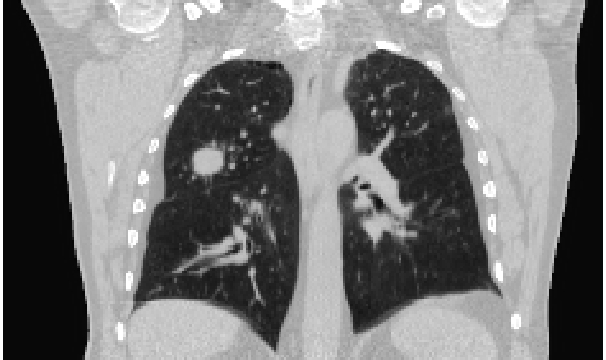
\includegraphics[width=6cm,height=40mm]{figures/phantomCT.jpg}
\caption{\DIFdelbeginFL \DIFdelFL{Illustration }\DIFdelendFL \DIFaddbeginFL \DIFaddFL{Coronal slice }\DIFaddendFL of the \DIFdelbeginFL \DIFdelFL{numerical phantom which is }\DIFdelendFL \DIFaddbeginFL \DIFaddFL{thorax CT }\DIFaddendFL used for this study\DIFdelbeginFL \DIFdelFL{and based on the patient CT acquisition}\DIFdelendFL . Tumour
  target is clearly visible \DIFaddbeginFL \DIFaddFL{in the center of the parenchyma }\DIFaddendFL on \DIFdelbeginFL \DIFdelFL{this illustrated slice}\DIFdelendFL \DIFaddbeginFL \DIFaddFL{the
  right lung (left of the image)}\DIFaddendFL .}
\label{fig00}
\end{figure}

\subsubsection{Physics list}

As recommended by the Geant4 Electromagnetic Standard working group
\DIFdelbegin \DIFdel{~}%DIFDELCMD < \cite{G4EMGroup2010} %%%
\DIFdelend for medical physics applications\DIFaddbegin \DIFadd{~}\cite{G4EMGroup2010}\DIFaddend , we used the
electromagnetic (EM) standard package with the option 3 (Opt3)
parameters-list. Regarding hadronic interactions, we followed the
recommendation of~\cite{Pshenichnov2007, Zacharatou2008}. One
difference was, following~\cite{Polf2009, Peterson2009,
  Grevillot2010}, that we used only the precompound model as inelastic
hadronic model even above 80 MeV (unlike~\cite{Pshenichnov2007}), that
have been found to be \DIFdelbegin \DIFdel{more close }\DIFdelend \DIFaddbegin \DIFadd{closer }\DIFaddend to measurement in proton
experiments. Very recently, Bohlen et al~\cite{Bohlen2010} proposed \DIFdelbegin \DIFdel{a very }\DIFdelend \DIFaddbegin \DIFadd{an
}\DIFaddend interesting study comparing nuclear fragmentation models of FLUKA and
Geant4 for carbon ion therapy, and gave indication to better tune
Geant4. Those recommendation will be included in future works.  In the
case of this study, we are focused on the positron emitter production
($^{11}$C and $^{15}$O) for dosimetry monitoring by PET imaging. As it
was demonstrated by Pshenichnov et al.~\cite{Pshenichnov2006} and
illustrates by the table\DIFaddbegin \DIFadd{~}\DIFaddend \ref{tab:CrossSection}, the numerical model
overestimates the cross section production for $^{11}$C and $^{15}$O
of 15\% to 20\%. This will be directly correlated to the PET signal
with an overestimation in the same range.

\begin{table}[htbp]
\begin{center}
  \begin{tabular}{|c|c|c|c|c|c|c|} \hline
    $^{12}$C energy  & \multicolumn{2}{|c|}{212.12 A MeV}  & \multicolumn{2}{|c|}{259.5 A MeV}  & \multicolumn{2}{|c|}{343.46 A MeV}       \\
    \cline{2-7} & Simulation & Experiment & Simulation & Experiment &
    Simulation & Experiment \\ \hline \hline 
    \DIFdelbeginFL %DIFDELCMD < 

%DIFDELCMD <  %%%
\DIFdelendFL $^{11}$C             & 11.9  &  10.5  &  16.8  &  14.7  &  25.25  &  19.9      \\ \hline
    $^{15}$O             & 2.38  &  2.1  &  3.69  &  3.1   &  6.09   &  5.0        \\ \hline \hline 

\end{tabular}
\end{center} 
\caption{\it Production yields of positron emitters in a PMMA phantom: Geant4/GATE simulation versus experimental data. \DIFaddbeginFL \dsnote{Quelle unité ?A indiquer }\DIFaddendFL } 
\label{tab:CrossSection}
\end{table}

\DIFaddbegin \dsnote{D'ou tiens tu ces valeurs ? Tes manips ? S'il c'est déjà
  publié dans un papier, pas la peine de le remttre me semble t il.}


\DIFaddend \subsubsection{Scanned beam delivery system}

We considered a virtual beam delivery system inspired from the one
described in~\cite{Kramer2000a}. Scanning is achieved with
superimposition of multiple carbon ion spots varying in lateral and
longitudinal directions, and in energy. The scanning is intended to
spread out the dose such that the target volume receive an uniform and
high dose.  Given a beam direction, the distal plane of the target
volume was sampled with spots positions every 1.5 mm. Each spot was
mono-energetic, have a symmetric Gaussian profile of 5 mm FWHM and was
directed towards its end point in the distal plane. We considered
energy layers every 2 mm (about 3 MeV). We defined a simple pencil
beam model following~\cite{Grevillot2010}. We considered a unique spot
size, even if generally, the size depends on the beam energy. More
advanced descriptions of a pencil beam scanning delivery technique can
be performed~\DIFdelbegin %DIFDELCMD < \cite{Grevillot2010} %%%
\DIFdelend \DIFaddbegin \cite{Grevillot2011} \DIFaddend when focus on a real facility. In
Carbon facilities, such as at HIT or GSI, the irradiation delivered by
the synchrotron is pulsed, with spills (beam extraction) during few
seconds (max 2 s) and spill period of about 5s, required for beam
injection and acceleration. We considered here a continuous time
structure and did not split it into spills. We did not also consider
the time required to switch energy between two iso-energy slices,
which is typically in the range of 1-2 s~\cite{Rietzel2010}. The
optimization of each spot intensity was performed according to the
simplified one-dimensional method of~\cite{Kramer2000a} in order to
obtain uniform dose in the target part. Optimization was performed
field by field \DIFaddbegin \DIFadd{(single field uniform dose, SFUD~}\cite{Lomax1999}\DIFadd{)}\DIFaddend . We
used a precomputed database of depth deposited energy profiles in
water. The database contained profiles with energy from 50 MeV/u to
490 MeV/u, with a 0.05 mm depth resolution and was computed with
multiple GATE simulations and stored in a database. Water Equivalent
Path Length (WEPL) were computed for all lines going from the virtual
beam source to each spot positions in the distal plane and
intersecting the CT voxels. Total WEPL was estimated by summing the
individual WEPL along all intersected voxels weighted by the
intersection length. WEPL for a given material was computed with an
approximation of the relative stopping power (to water) computed with
the Bethe-Bloch formula: $wepl = \rho \frac{Z/A}{0.555}$, with Z and A
the atomic and mass number of the material.
\DIFdelbegin %DIFDELCMD < \\
%DIFDELCMD < %%%
\DIFdelend \DIFaddbegin 

\DIFaddend In the case of this study, we considered 3 fields leading to almost
6000 individual spots. It does not correspond to real treatment plans
but aims at describing representative test case. Three \DIFdelbegin \DIFdel{set-up }\DIFdelend \DIFaddbegin \DIFadd{setup }\DIFaddend of
primary carbon ions flux were launched. Typical irradiation-dose rate
is 5 GyE/min/l~\cite{Noda2007}, corresponding to an intensity of
$1.2\times 10^9$ pps (particles per seconds). Regarding our simplified
pencil beam description, we thus considered that in a range of $10^8$
to $10^9$ particles reach the patient will correspond to 1 Gy to 10 Gy
at the tumour. Table\DIFaddbegin \DIFadd{~}\DIFaddend \ref{tab:setup} shows the beam \DIFdelbegin \DIFdel{set-up }\DIFdelend \DIFaddbegin \DIFadd{setup }\DIFaddend for the 3
configurations.

\begin{table}[htbp]
\begin{center}
\begin{tabular}{|c|c|c|} \hline
Simulation \DIFdelbeginFL \DIFdelFL{set-up }\DIFdelendFL \DIFaddbeginFL \DIFaddFL{setup }\DIFaddendFL name  & $^{12}$C number  & Tumour dose (Gy)       \\\hline \hline

$S_{1}$    & $3.10^{8}$             & 1                                          \\ \hline
$S_{2}$    & $15.10^{8}$                  & 5                                          \\ \hline
$S_{3}$    & $3.10^{9}$                 & 10                                      \\ \hline \hline 

\end{tabular}
\end{center} 
\caption{\it \DIFdelbeginFL \DIFdelFL{Set-up }\DIFdelendFL \DIFaddbeginFL \DIFaddFL{Setup }\DIFaddendFL description: Carbon ions beam \DIFdelbeginFL \DIFdelFL{versus }\DIFdelendFL \DIFaddbeginFL \DIFaddFL{and }\DIFaddendFL target dose.}
\DIFdelbeginFL %DIFDELCMD < \label{tab:results}
%DIFDELCMD < %%%
\DIFdelendFL \DIFaddbeginFL \label{tab:setup}
\DIFaddendFL \end{table}



%dose relat / absolue ; no RBE (?) mentionner LET is available in each voxel
%=> chercher dose max par fraction (pas en GyE)
%cf url send to Seb

%http://totlxl.to.infn.it/mediawiki/index.php?title=Water_equivalent_path_length
% **IMAGE OF ALL BP**
% dsarrut@oronge:~/src/tinytps/BeamLines/RBE1
%% ~/src/tinytps/Simulations/Test2

%~/recherche/grandChallenge/simulations/lung/mac_patient2_3> 
% grep "/gps/source/add" spots1-lung.mac | wc -l 1973
% grep "/gps/source/add" spots2-lung.mac | wc -l 1937
% grep "/gps/source/add" spots3-lung.mac | wc -l 2034

% The two beam descriptions (beam1.mac and beam2.mac) used into
% main.mac, correspond to the physical dose SOBP optimization. The file
% beamRBE.mac corresponds to the results of a SOBP optimization perform
% with a single field on biological dose computed with [Kase2006]
% method.

\subsubsection{Scorers}

Dose was scored with the GateDoseActor described
in~\DIFdelbegin %DIFDELCMD < \cite{Jan2010,Sarrut2008} %%%
\DIFdel{which store }\DIFdelend \DIFaddbegin \cite{Jan2011,Sarrut2008} \DIFadd{that stores }\DIFaddend deposit dose and energy
distribution in a 3D matrix of dosels, together with the associated
statistical uncertainty. We choose a matrix of dosels of size \DIFdelbegin \DIFdel{$2\times 2 \times 2 mm^3$}\DIFdelend \DIFaddbegin \DIFadd{$2^3
mm^3$}\DIFaddend .  We also stored the 3D distribution of \DIFdelbegin \DIFdel{point }\DIFdelend \DIFaddbegin \DIFadd{points }\DIFaddend of creation of
$\beta^+$ emitters during the irradiation. We limited emitters scoring
to the two main ones, $^{11}C$ and $^{15}O$~\cite{Pshenichnov2007},
the others ($^{10}C$, $^{13}N$, $^{14}O$, $^{17,18}F$, $^{30}P$, for
those with more than 10 s of half-live) were considering to have
negligible influence on a reconstructed PET image but could also be
stored if needed. \DIFdelbegin %DIFDELCMD < \\ 
%DIFDELCMD < %%%
%DIF < \textbf{SEB : est ce que la dose (faible?) d{\'e}pos{\'e}e par ces emitters est prise
%DIF < en compte ? A indiquer ici}
\DIFdelend The energy deposited by secondary particles and
specially by $\beta^+$ emitters in this case, \DIFdelbegin \DIFdel{is }\DIFdelend \DIFaddbegin \DIFadd{was }\DIFaddend taking into account
in the dose and energy 3D \DIFdelbegin \DIFdel{matrix}\DIFdelend \DIFaddbegin \DIFadd{matrices}\DIFaddend .

%DIF > \textbf{SEB : est ce que la dose (faible?) d{\'e}pos{\'e}e par ces emitters est prise
%DIF > en compte ? A indiquer ici} YES.
\DIFaddbegin 

\DIFaddend %to compare to [attanasi 2009] (events collected during 6 times 10 Gy.)

\subsection{Simulation \DIFdelbegin \DIFdel{set-up}\DIFdelend \DIFaddbegin \DIFadd{setup}\DIFaddend : PET scan for dose monitoring}

The PET acquisition \DIFdelbegin \DIFdel{modelling }\DIFdelend \DIFaddbegin \DIFadd{modeling }\DIFaddend is the second part of the complete
simulation \DIFdelbegin \DIFdel{set-up. It 's }\DIFdelend \DIFaddbegin \DIFadd{setup. It is }\DIFaddend not an in-beam PET configuration\DIFdelbegin \DIFdel{which explain that }\DIFdelend \DIFaddbegin \DIFadd{: }\DIFaddend there is no
\DIFdelbegin \DIFdel{contamination by the gamma prompts emission }\DIFdelend \DIFaddbegin \DIFadd{prompt gamma contamination }\DIFaddend during the acquisition.

\subsubsection{Scanner description}

The \DIFdelbegin \DIFdel{scanner modelled }\DIFdelend \DIFaddbegin \DIFadd{modeled scanner }\DIFaddend for this study is the \DIFdelbegin \DIFdel{commerdial }\DIFdelend \DIFaddbegin \DIFadd{commercial }\DIFaddend ECAT EXACT
HR+~\cite{Brix1997} system by Siemens. This scanner is made of four
rings of BGO blocks partially cut into an 8x8 array of crystals
measuring 4.0x4.1x30 mm$^3$ each, resulting in a 82.7 cm diameter
detector cylinder and an axial field-of-view (\DIFdelbegin \DIFdel{F.O.V.}\DIFdelend \DIFaddbegin \DIFadd{FOV}\DIFaddend ) length of 15.5
cm. \DIFdelbegin \DIFdel{Figure~\ref{fig:fig0} shows the global geometry description of the HR+ scanner with GATE in the 3D acquisition mode where we }\DIFdelend \DIFaddbegin \DIFadd{We }\DIFaddend defined the BGO blocks, a back compartment to simulate the back
scattering induced by the light collection system, the lead
end-shielding, and the patient bed. \DIFaddbegin \DIFadd{Figure~\ref{fig:fig0} illustrates
the global geometry of the HR+ scanner. }\DIFaddend The simulation assumes an
energy resolution for each crystal randomly drawn from a uniform
distribution varying between $20 \%$ and $30 \%$ at 511 keV. The
determination of the hit crystal is based on the crystal with the
highest energy deposition, to which an additional analytical spatial
blurring based on a 2D Gauss kernel can be applied to model the
decrease induced by the photomultiplier tube Anger electronic
system. A global sensitivity factor is also defined for each block to
replicate the sensitivity performance of the scanner; this efficiency
factor is set at $90 \%$ in the case of the HR+. As for the
experimental data, a 350-650 keV energy window and a 12 ns coincidence
time window were applied. This PET scanner was already modelled and
validated by using GATE and all results are described
in~\cite{Jan2005}.

\begin{figure}[!h]
\centering
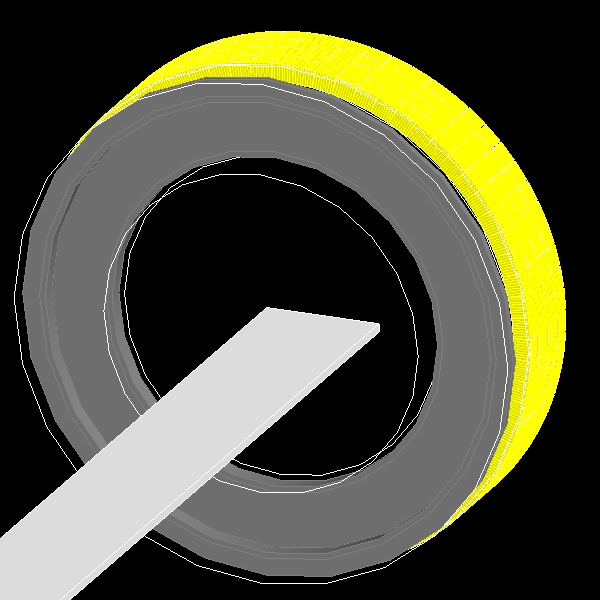
\includegraphics[width=40mm,height=40mm]{figures/HR_Simu_Gate_GC.jpg}
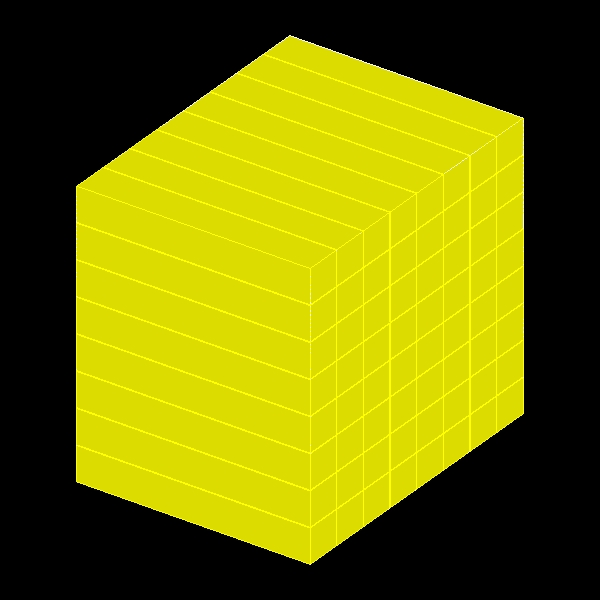
\includegraphics[width=40mm,height=40mm]{figures/bloc_detec_HR.jpg}
\caption{Illustration of the \DIFaddbeginFL \DIFaddFL{HR+ }\DIFaddendFL PET scanner simulated with GATE
  \DIFdelbeginFL \DIFdelFL{and }\DIFdelendFL \DIFaddbeginFL \DIFaddFL{(Left). At right, }\DIFaddendFL one of the 288 \DIFdelbeginFL \DIFdelFL{bloc }\DIFdelendFL \DIFaddbeginFL \DIFaddFL{blocks }\DIFaddendFL PET detectors which is
  composed by 64 BGO crystals\DIFdelbeginFL \DIFdelFL{for the Siemens HR+
scanner}\DIFdelendFL \DIFaddbeginFL \DIFaddFL{. }\dsnote{C'est pas très beau ... (si je
    peux me permettre). Allez, un effort, tu peux faire un truc qui
    pete non ? }\DIFaddendFL }
\label{fig:fig0}
\end{figure}

\subsubsection{Data treatments and image reconstruction}

To improve the data quantification, the simulated data \DIFdelbegin \DIFdel{are }\DIFdelend \DIFaddbegin \DIFadd{were
}\DIFaddend normalized, attenuated corrected and reconstructed using the 3D OSEM
method~\DIFdelbegin %DIFDELCMD < \cite{OSEM ref}%%%
\DIFdelend \DIFaddbegin \cite{OSEM_ref}\DIFaddend . To speed-up the complete processing, we used a
PET analytic simulator, ASIM~\cite{Comtat1999}, with the ECAT HR+
scanner geometry description to produce the normalization
sinogram. For the attenuation correction, coefficient factors (ACFs)
\DIFdelbegin \DIFdel{are }\DIFdelend \DIFaddbegin \DIFadd{were }\DIFaddend also calculated with ASIM using the voxelized attenuation map
description provided by the numerical patient phantom.

\subsection{Running GATE on a High Performance Computing machine}

These simulations were running at the French Rechearch and Technology
Computing Center~\cite{CCRT} on the TITANE supercomputer. This is a
cluster integrating 1596 Bull NovaScale R422 servers, with 2 Intel
Xeon 5570 quad core processors each including a memory of 3 Go per
core. With 3192 Intel Xeon 5570 4 cores, TITANE offers a processing
capacity \DIFdelbegin \DIFdel{in excess of }\DIFdelend \DIFaddbegin \DIFadd{above }\DIFaddend 90 teraflops, and 25 terabytes of core memory, which
put it in june 2009 in 38th place of the worldwide supercomputer sites
Top500 ranking. The TITANE cluster operates the Bull HPC software
platform that includes the Linux operating system and the global and
parallel Lustre file system. This platform is based on an open source
software integrated and optimized by Bull's HPC competence center in
Echirolles, France. \DIFaddbegin \DIFadd{GATE simulations were split into similar jobs
having different random seeds. Because it is a dedicated
supercomputer, we used a static parallelization, each job tracking the
same number of particles~}\cite{Camarasu-Pop2010}\DIFadd{.
}\DIFaddend 

%%%%%%%%%%%%%%%%%%%%%%%%%%%%%%%%%%%%%%%%%%%%%%%%%%%%%%
\section{Results and discussion}

%All figures are presented with the same dynamic in the look up table.
%Averaged statistical uncertainty was close to $XX\%$ for all dosel with more than $50\%$ of the maximum deposited
%dose~\cite{Chetty2006b}.\\ % <---- TO PUT IN RESULTS ???


The figure~\ref{fig:fig1} shows the dose deposited during \DIFaddbegin \DIFadd{the
}\DIFaddend irradiation and the $\beta^+$ emitter maps for $^{11}$C and $^{15}$O
isotopes which are produced by $^{12}$C interactions for the \DIFdelbegin \DIFdel{protocol }\DIFdelend \DIFaddbegin \DIFadd{setup }\DIFaddend S3
where 10 Gy were deposited on the tumour. These images are \DIFdelbegin \DIFdel{the }\DIFdelend \DIFaddbegin \DIFadd{a
}\DIFaddend qualitative proof of concept of the GATE capabilities to perform
complete and realistic simulations in the field of hadrontherapy
coupled with a nuclear imaging device.

\begin{figure}[!h]
  \centering
  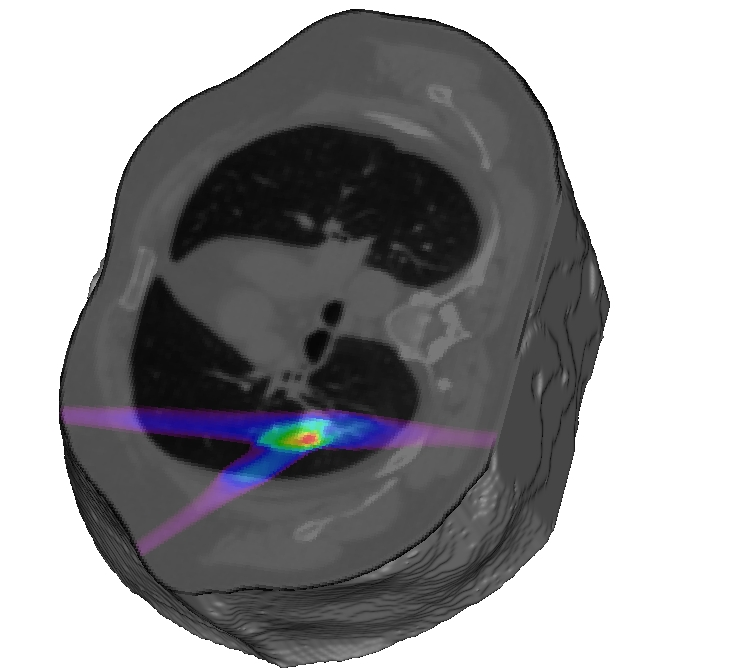
\includegraphics[width=55mm,height=35mm]{figures/3D-Dose_poumon.jpg}\DIFaddbeginFL \\
  \DIFaddendFL 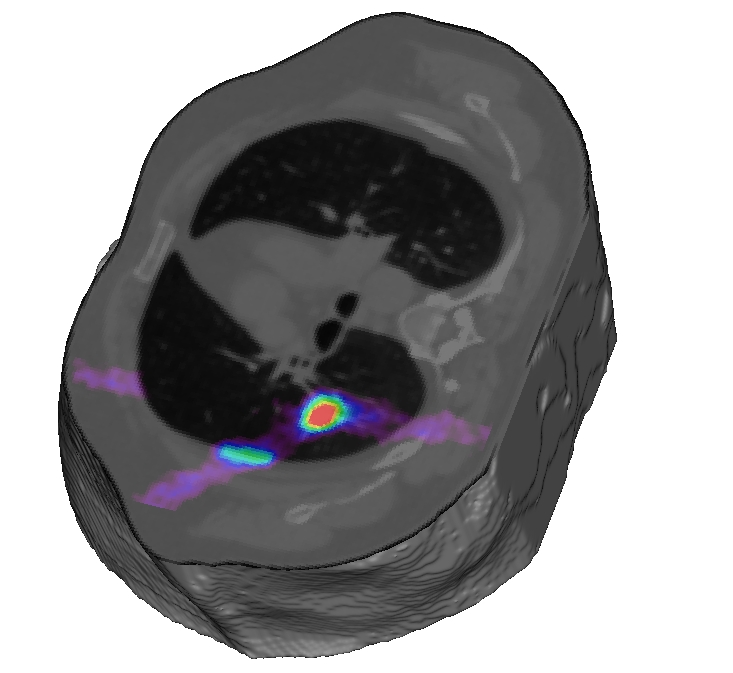
\includegraphics[width=55mm,height=35mm]{figures/3D-PETC11_poumon.jpg}
  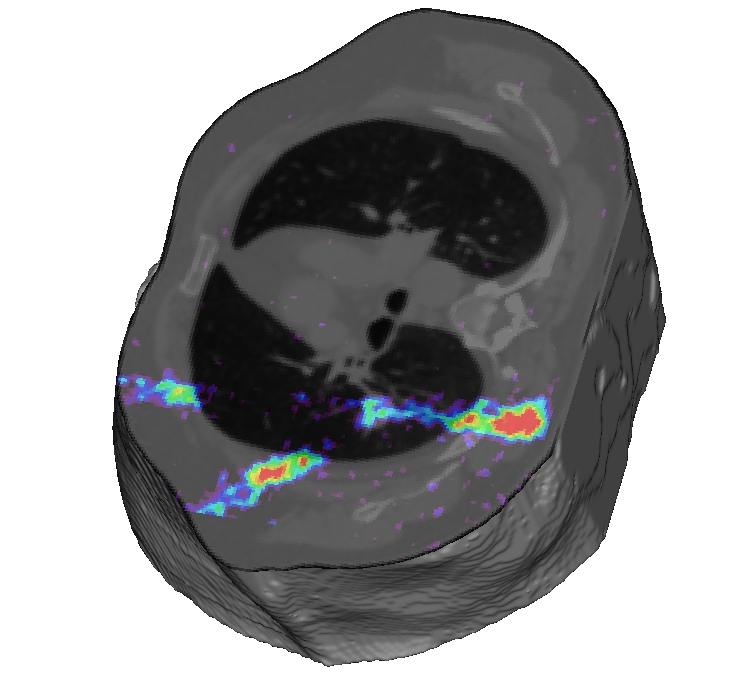
\includegraphics[width=55mm,height=35mm]{figures/3D-PETO15_poumon.jpg}
  \caption{Lung dose deposition \DIFdelbeginFL \DIFdelFL{- }\DIFdelendFL \DIFaddbeginFL \DIFaddFL{(Top), and }\DIFaddendFL PET $^{11}$C - PET $^{15}$O
    \DIFaddbeginFL \DIFaddFL{emitter distribution map (Bottom).}\DIFaddendFL }

\label{fig:fig1}
\end{figure}

To \DIFdelbegin \DIFdel{validate }\DIFdelend \DIFaddbegin \DIFadd{illustrate }\DIFaddend the interest to model the complete \DIFdelbegin \DIFdel{scheme }\DIFdelend \DIFaddbegin \DIFadd{process, }\DIFaddend from the
radiation to the scanner acquisition system, we \DIFdelbegin \DIFdel{have }\DIFdelend compared the final
\DIFdelbegin \DIFdel{image }\DIFdelend \DIFaddbegin \DIFadd{images }\DIFaddend with and without a dedicated model of the PET camera. The \DIFdelbegin \DIFdel{figure~\ref{fig:fig2} shows what we can find in the literature: the PET scanner is modelled }\DIFdelend \DIFaddbegin \DIFadd{first
row in figure~\ref{fig:fig3} shows the PET image modeled }\DIFaddend by using a
smoothing spatial Gaussian function applied \DIFdelbegin \DIFdel{on }\DIFdelend \DIFaddbegin \DIFadd{to }\DIFaddend the $\beta^{+}$
emitters distribution maps\DIFaddbegin \DIFadd{, such as for example done
in~}\cite{Parodi2007a}\DIFaddend . This approach does not take into account
\DIFdelbegin \DIFdel{some }\DIFdelend important physical effects \DIFdelbegin \DIFdel{like }\DIFdelend \DIFaddbegin \DIFadd{such as }\DIFaddend positron range in tissue, material
attenuation, photon scattering and the sensitivity of the PET camera
including the detection solid angle and the intrinsic detector
response. All these effects have an impact on the image quality and
finally on the dose quantification with a PET acquisition. The
difference is clearly \DIFdelbegin \DIFdel{demonstrated }\DIFdelend \DIFaddbegin \DIFadd{visible }\DIFaddend when we compare the images \DIFdelbegin \DIFdel{on figure~\ref{fig:fig2} and what we }\DIFdelend \DIFaddbegin \DIFadd{with the ones
}\DIFaddend obtained with the protocol $S_{3}$\DIFaddbegin \DIFadd{, }\DIFaddend illustrated by the \DIFaddbegin \DIFadd{two first rows
of }\DIFaddend figure~\ref{fig:fig3} where the PET camera is \DIFdelbegin \DIFdel{modelled}\DIFdelend \DIFaddbegin \DIFadd{modeled}\DIFaddend . Without PET
camera \DIFdelbegin \DIFdel{modelling}\DIFdelend \DIFaddbegin \DIFadd{modeling}\DIFaddend , the quality and image contrast with a dose delivery
of 1 Gy in the target is higher than what we can obtained with 10 Gy
in the same protocol which includes the PET camera model. This result
demonstrates that data quantification is not realistic with a
simplified approach of the imaging system.

\DIFaddbegin \dsnote{C'est S3 ou S1 pour le Gaussian ?}

\dsnote{Est ce qu'on peut mettre un critere quantitatif ? }

%DIF >  \begin{figure}[!h]
%DIF >  \centering
%DIF >  \caption{$^{11}$C and $^{15}$O PET images using a spatial smoothing Gaussian function for PET scanner modelling in the case of 1 Gy deposited at the tumour level}
%DIF >  \label{fig:fig2}
%DIF >  \end{figure}

\DIFaddend \begin{figure}[!h]
  \centering
  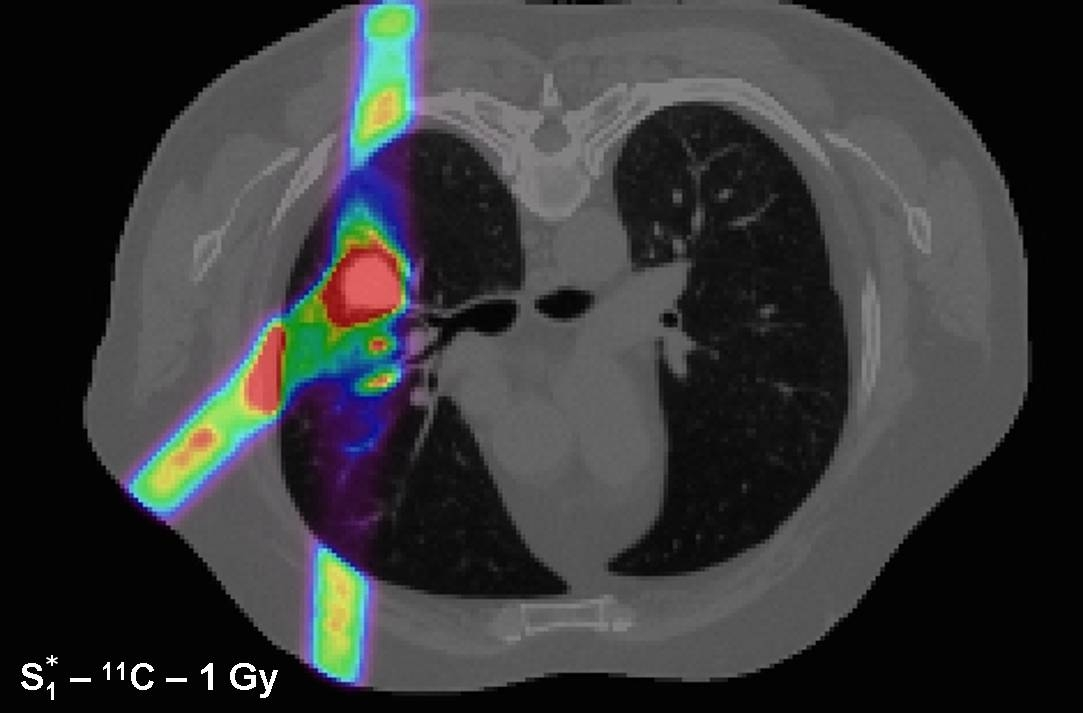
\includegraphics[width=6cm,height=40mm]{figures/gaussPET_C11_v1.jpg}
  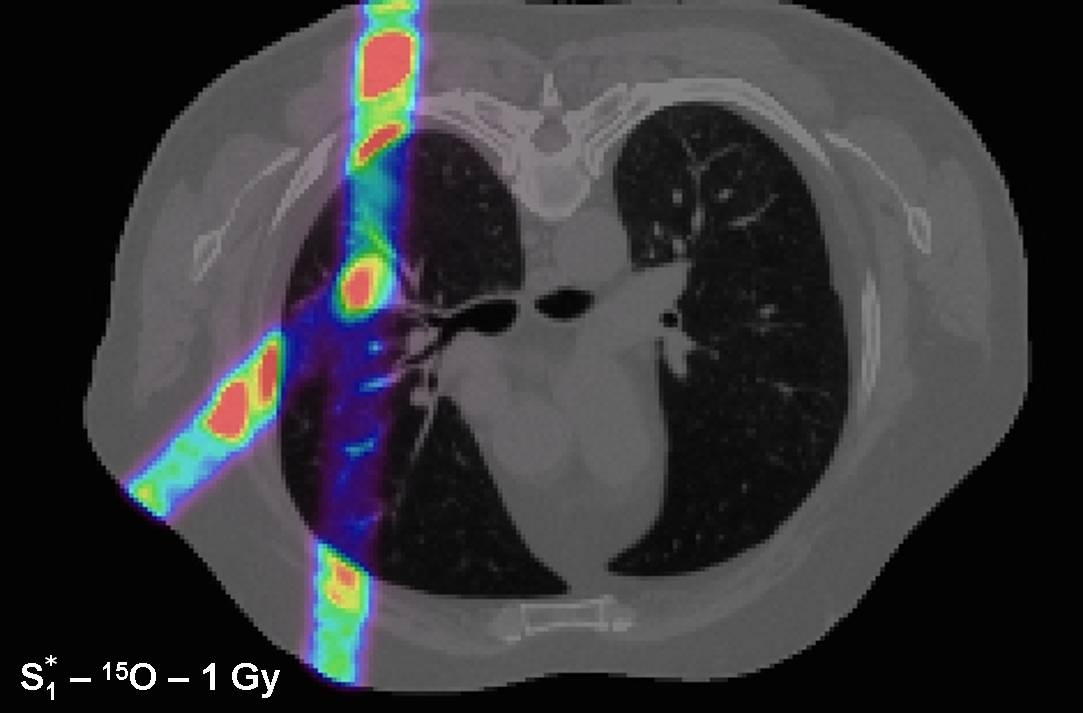
\includegraphics[width=6cm,height=40mm]{figures/gaussPET_O15_v1.jpg}
  \DIFdelbeginFL %DIFDELCMD < \caption{%
{%DIFAUXCMD
\DIFdelFL{$^{11}$C and $^{15}$O PET images using a spatial smoothing Gaussian function for PET scanner modelling in the case of 1 Gy deposited at the tumour level}}
%DIFAUXCMD
%DIFDELCMD < \label{fig:fig2}
%DIFDELCMD < \end{figure}
%DIFDELCMD < 

%DIFDELCMD < \begin{figure}[!h]
%DIFDELCMD < \centering
%DIFDELCMD < %%%
\DIFdelendFL 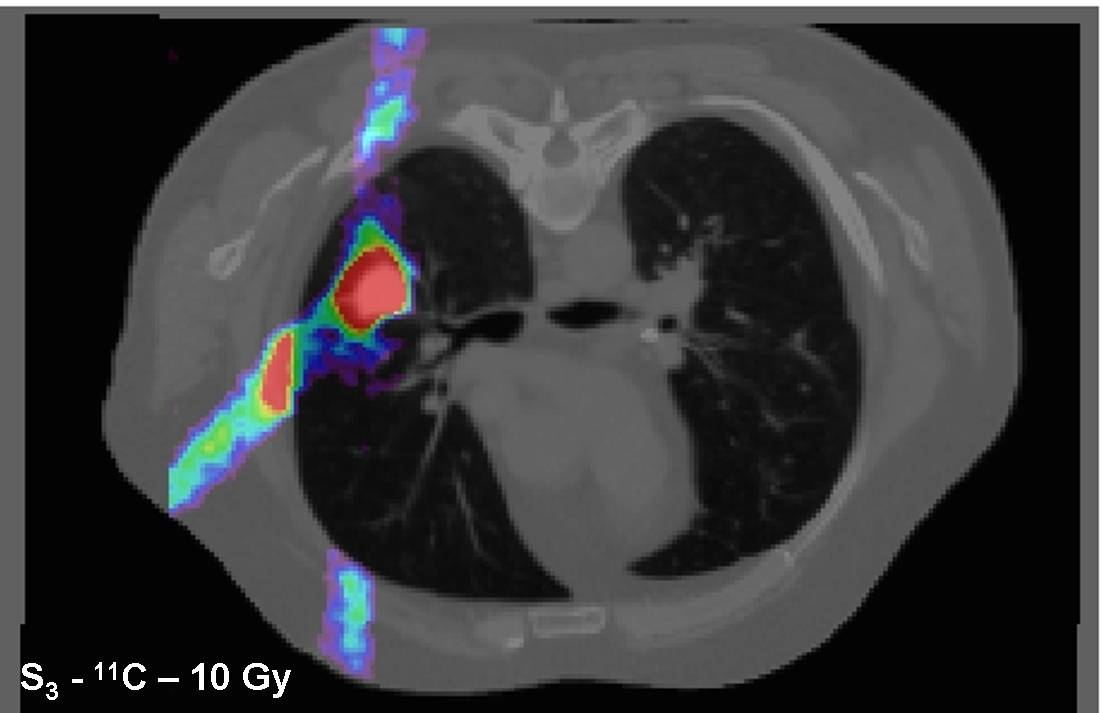
\includegraphics[width=6cm,height=40mm]{figures/C11_10Gy_v1.jpg}
  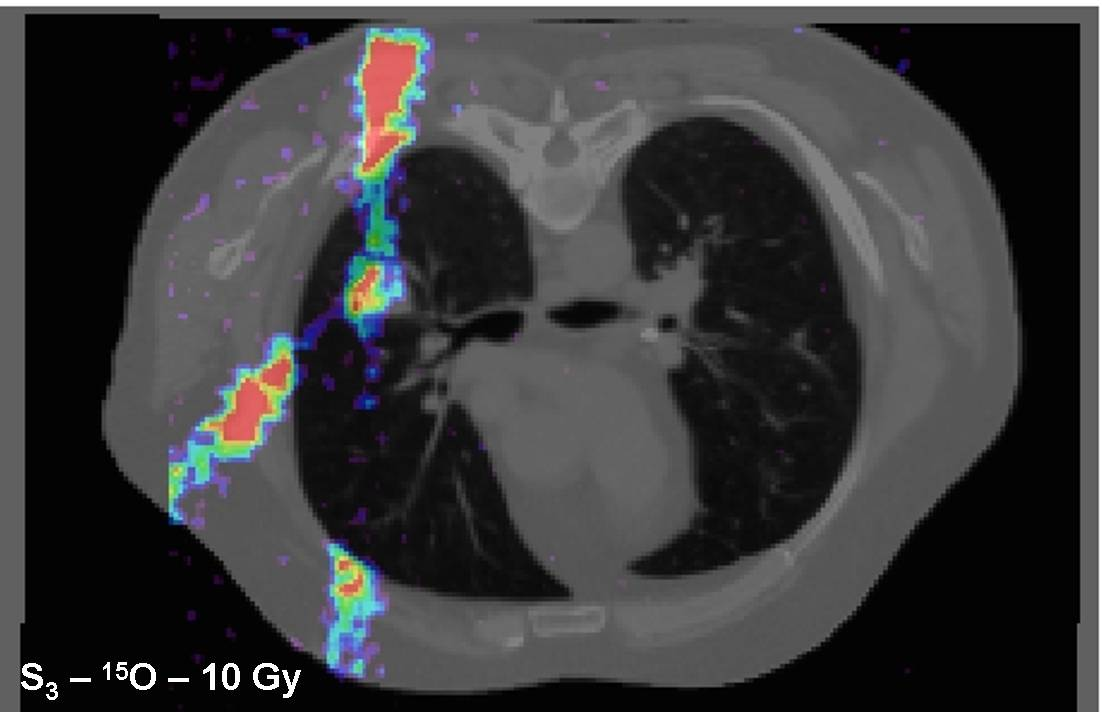
\includegraphics[width=6cm,height=40mm]{figures/O15_10Gy_v1.jpg}
  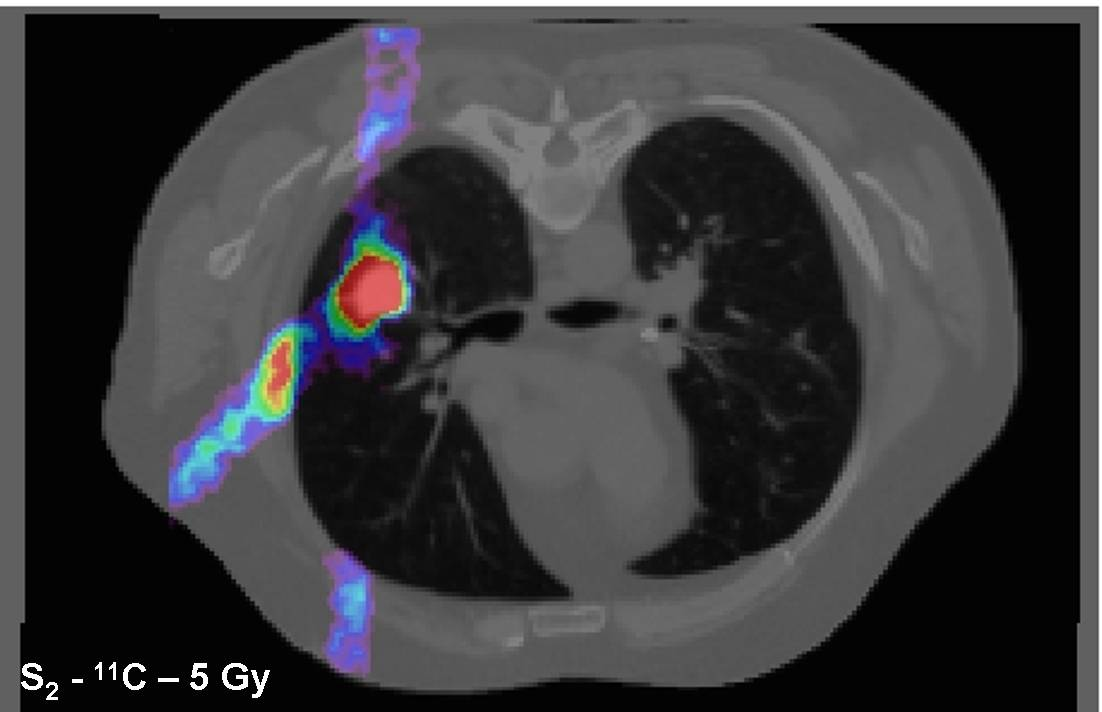
\includegraphics[width=6cm,height=40mm]{figures/C11_5Gy_v1.jpg}
  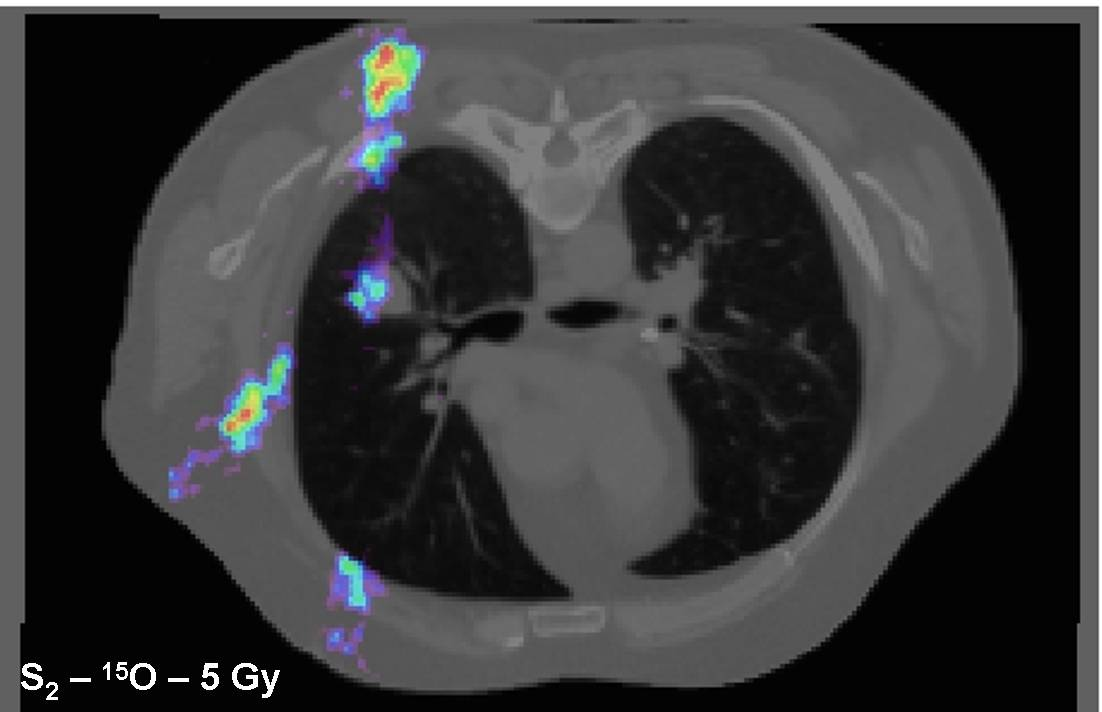
\includegraphics[width=6cm,height=40mm]{figures/O15_5Gy_v1.jpg}
  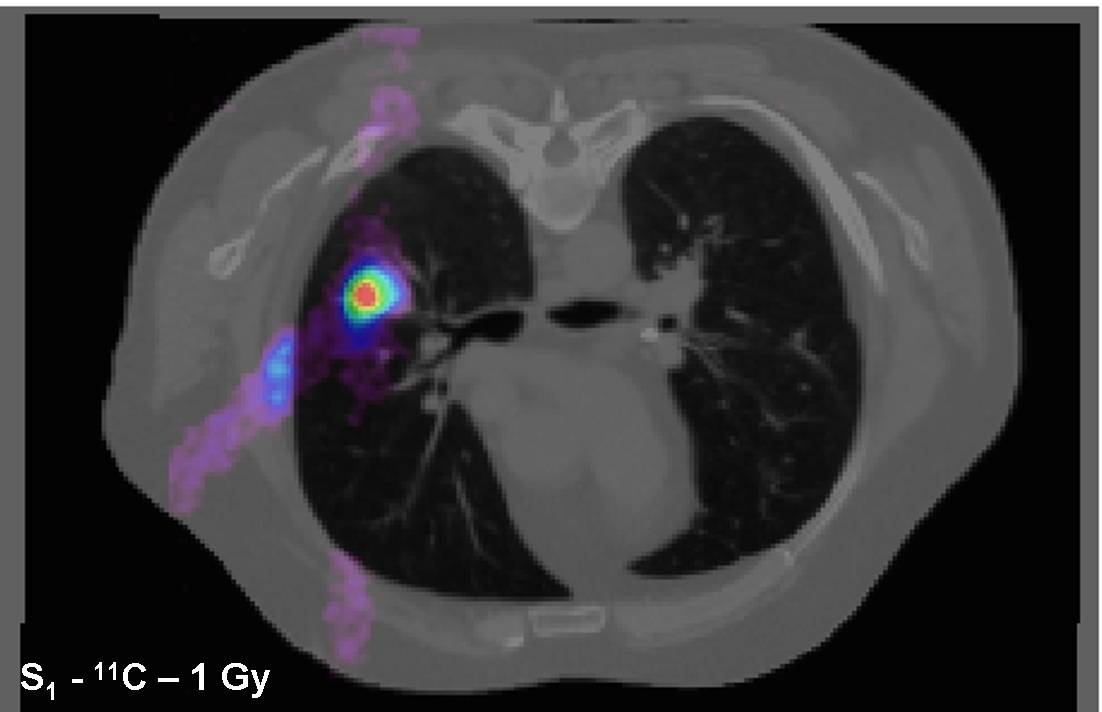
\includegraphics[width=6cm,height=40mm]{figures/C11_1Gy_v1.jpg}
  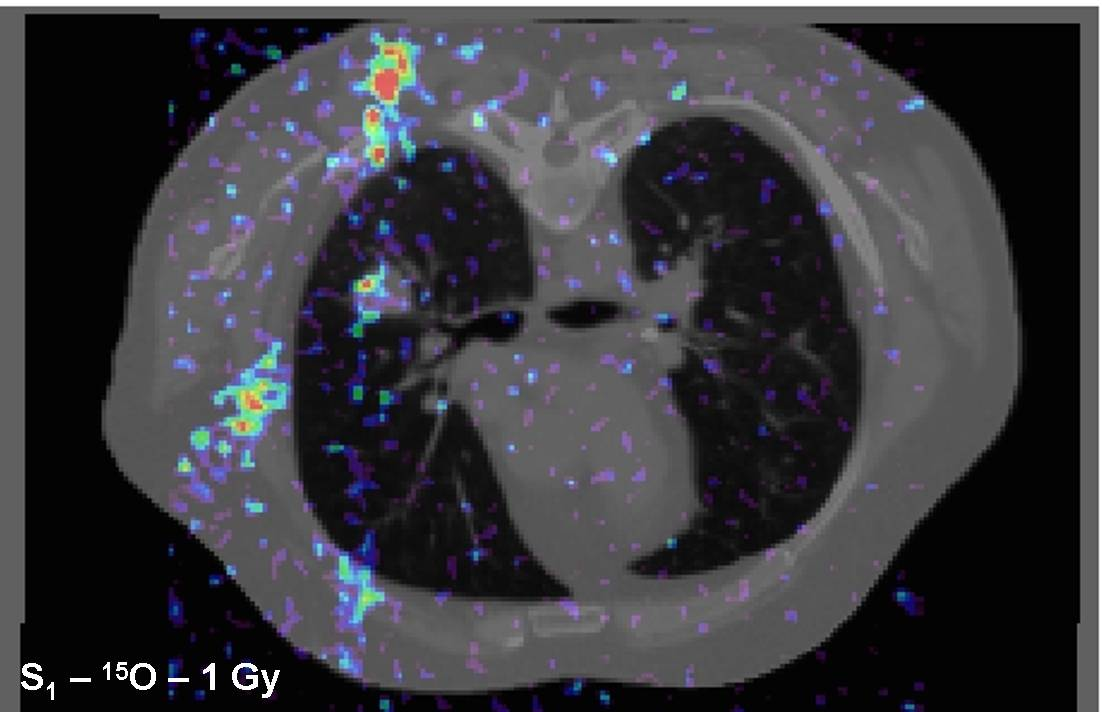
\includegraphics[width=6cm,height=40mm]{figures/O15_1Gy_v1.jpg}
  \caption{\DIFdelbeginFL \DIFdelFL{Statistic distribution for PET }\DIFdelendFL \DIFaddbeginFL \DIFaddFL{The first row depicts }\DIFaddendFL $^{11}$C \DIFaddbeginFL \DIFaddFL{(left) }\DIFaddendFL and \DIFdelbeginFL \DIFdelFL{PET }\DIFdelendFL $^{15}$O \DIFdelbeginFL \DIFdelFL{acquisition with 10 Gy }\DIFdelendFL (\DIFaddbeginFL \DIFaddFL{right)
    PET images using a spatial smoothing Gaussian function for the
    }\DIFaddendFL S$_{3}$ \DIFaddbeginFL \DIFaddFL{setup. The other rows show statistic distributions
    obtained from the complete imaging simulation for setup S$_{3}$
    (10 Gy}\DIFaddendFL ), \DIFdelbeginFL \DIFdelFL{5 Gy (}\DIFdelendFL S$_{2}$ \DIFaddbeginFL \DIFaddFL{(5 Gy}\DIFaddendFL ) and \DIFdelbeginFL \DIFdelFL{1 Gy (}\DIFdelendFL S$_{1}$ \DIFaddbeginFL \DIFaddFL{(1Gy}\DIFaddendFL )\DIFdelbeginFL \DIFdelFL{deposited at the tumour level}\DIFdelendFL \DIFaddbeginFL \DIFaddFL{.}\DIFaddendFL }
  \label{fig:fig3}
\end{figure}
\DIFaddbegin 

\DIFaddend An other point \DIFdelbegin \DIFdel{that we can discussed, is relative to }\DIFdelend \DIFaddbegin \DIFadd{of interest concerns }\DIFaddend the $^{15}$O isotope contribution
in the PET images of $^{11}$C distribution\DIFdelbegin \DIFdel{. Or with other words, }\DIFdelend \DIFaddbegin \DIFadd{: }\DIFaddend is it necessary to develop
a dedicated method to correct the $^{11}$C PET image from the $^{15}$O
contribution ? As \DIFdelbegin \DIFdel{precised }\DIFdelend \DIFaddbegin \DIFadd{shown }\DIFaddend in the table~\ref{tab:CrossSection} the
$^{11}$C production is higher than $^{15}$O by a factor \DIFdelbegin \DIFdel{4 or 5 between with the
}\DIFdelend \DIFaddbegin \DIFadd{4-5 with the
used }\DIFaddend $^{12}$C beam\DIFdelbegin \DIFdel{characteristics on this set-up}\DIFdelend . The isotope half-life is also an important
parameter to estimate the $^{15}$O contribution on the PET image
analysis: 2 minutes for $^{15}$O \DIFdelbegin \DIFdel{against }\DIFdelend \DIFaddbegin \DIFadd{vs }\DIFaddend 20 minutes for $^{11}$C. If we
take into account these 2 effects, with a PET acquisition of 10
minutes (post-irradiation), there is a factor 70 in the production
rate between the 2 isotopes. This is illustrated by the
figure~\ref{fig:fig5} \DIFaddbegin \DIFadd{showing the additional contribution for the both
isotopes, }\DIFaddend where it is clear\DIFaddbegin \DIFadd{, compare to second row in
figure~\ref{fig:fig3}, }\DIFaddend that the quantitative analysis of the location
and the dose deposited on the target will not be constrained by the
presence of multi $\beta^+$ emitters and specially by the $^{15}$O.

\DIFdelbegin %DIFDELCMD < \begin{figure}[!h]
%DIFDELCMD < %%%
\DIFdelend \DIFaddbegin \dsnote{How do you obtain 70 ? Explain in the text}

\dsnote{Fig no very illustrative : to compare with an other one, or
  give quantitative criteria}


\begin{figure}[!htbp]
  \DIFaddendFL \begin{center}
    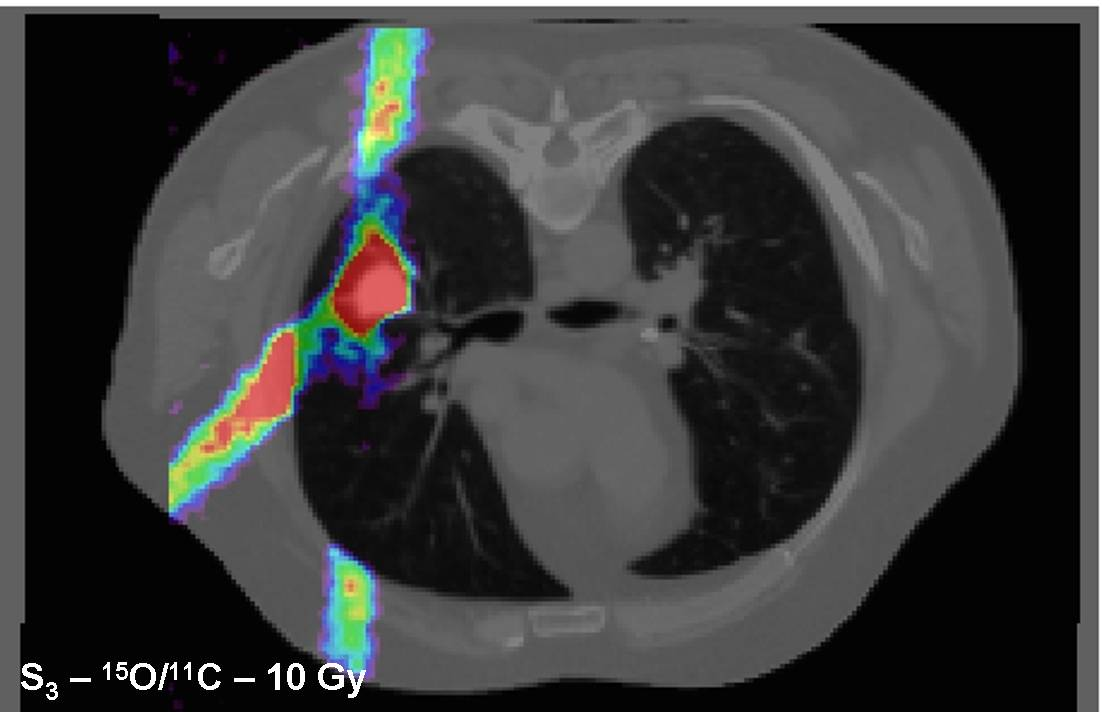
\includegraphics[width=6cm,height=40mm]{figures/C11_O15_10Gy_v1.jpg}
    \caption{PET image for the \DIFdelbeginFL \DIFdelFL{S3 scenario }\DIFdelendFL \DIFaddbeginFL \DIFaddFL{$S_3$ setup }\DIFaddendFL including the two \DIFdelbeginFL \DIFdelFL{isotope }\DIFdelendFL \DIFaddbeginFL \DIFaddFL{isotopes
      }\DIFaddendFL contribution: $^{11}$C and $^{15}$O\DIFaddbeginFL \DIFaddFL{.}\DIFaddendFL }
  \end{center}
  \label{fig:fig5}
\end{figure} 

\DIFdelbegin \DIFdel{The profiles illustrated by the figure~\ref{fig:fig4} allow us to assess the potential for quantification of PET imaging in }\DIFdelend \DIFaddbegin \DIFadd{Figure~\ref{fig:fig4} depicts the $^{11}$C and $^{15}$O normalized
counts as a }\DIFaddend function of the \DIFdelbegin \DIFdel{dose deposited in the tumour. These profiles are made on the most active distribution areaof the $\beta^+$ isotopes: the tumour for the $^{11}$C and thoracic tissue for $^{15}$O. It is clear that the dose of }\DIFdelend \DIFaddbegin \DIFadd{depth, for a line along the beam direction
passing to the tumor area. }\DIFaddend 1 Gy in the target seems to \DIFdelbegin \DIFdel{define the minimal
}\DIFdelend \DIFaddbegin \DIFadd{be the minimal
required }\DIFaddend dose for PET imaging quantification \DIFdelbegin \DIFdel{on this kind of protocol}\DIFdelend \DIFaddbegin \DIFadd{for the proposed
protocols}\DIFaddend . Table~\ref{tab:results} summarizes the main protocol
parameters to illustrate whether a therapeutic control with PET
imaging is feasible.

\DIFdelbegin %DIFDELCMD < \begin{figure}[!h]
%DIFDELCMD < %%%
\DIFdelend \DIFaddbegin \dsnote{Draw the depth line on the image.}

\dsnote{Your conclusion is not clear to me, at least not well
  supported. Tu dis que 1 Gy c'est le minimal et indique 'no' dans le
  table ? Il faudrait un critere quantitatif. Est ce qu'on peut
  mesurer le bruit de l'image TEP ? Ou la correlation avec la dose ?}

\begin{figure}[!htbp]
  \DIFaddendFL \begin{center}
    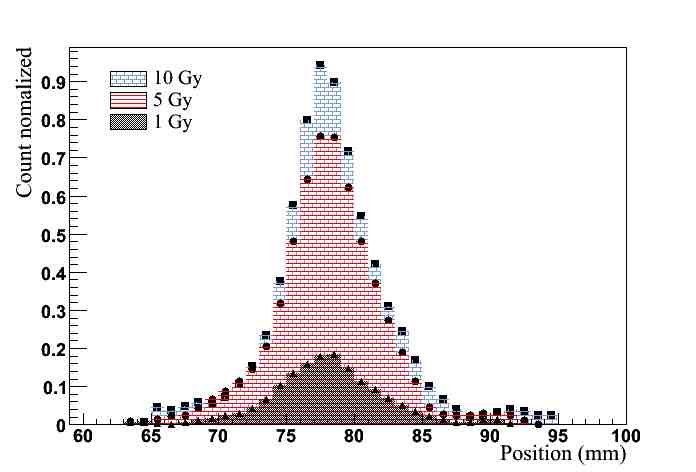
\includegraphics[width=75mm,height=55mm]{figures/histo_lung_C11_paper.jpg}
    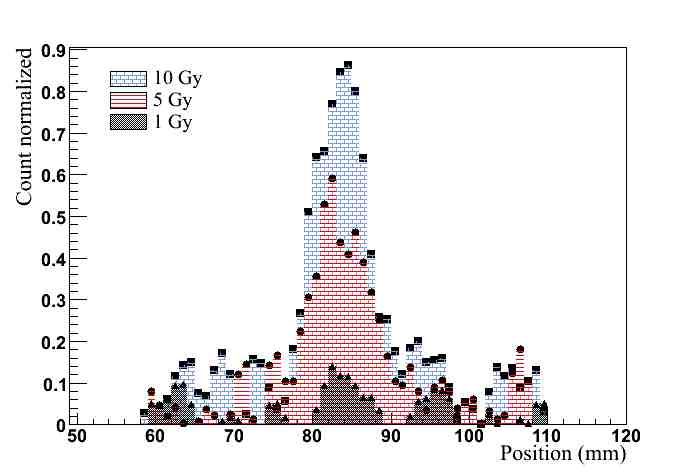
\includegraphics[width=75mm,height=55mm]{figures/histo_lung_O15_paper.jpg}
    \caption{Histogram distribution for quantitative analysis on PET
      images versus dose deposited at the tumour level - Histogram
      based on the tumour profile for the $^{11}$C distribution and on
      the thoracic tissue for $^{15}$0.}
  \end{center}
  \label{fig:fig4}
\end{figure}

\begin{table}[htbp]
\begin{center}
\begin{tabular}{|c|c|c|} \hline
 Protocol Name  & PET acquisition time  & PET image quantification       \\
                              &  min                  & of $\beta^{+}$ emitter distribution       \\ \hline \hline

$S_{3}$              & 10                    &  yes                           \\ \hline
$S_{2}$              & 10                    &  yes                           \\ \hline
$S_{1}$              & 10                    &  no                            \\ \hline \hline 

\end{tabular}
\end{center} 
\caption{\it Relation between the tumour deposited dose and the $^{11}$C PET image monitoring.}
\label{tab:results}
\end{table}


%%%%%%%%%%%%%%%%%%%%%%%%%%%%%%%%%%%%%%%%%%%%%%%%%%%%%%%%%%%%%%%%%%%%%%%%%%%%%%%%%%%%%%%
\DIFaddbegin \clearpage
\DIFaddend \section{Conclusion}

This study demonstrates the capability \DIFdelbegin \DIFdel{to perform with GATE some very }\DIFdelend \DIFaddbegin \DIFadd{of GATE to perform }\DIFaddend realistic
simulations in the \DIFdelbegin \DIFdel{field }\DIFdelend \DIFaddbegin \DIFadd{fields }\DIFaddend of hadrontherapy and nuclear imaging\DIFdelbegin \DIFdel{for }\DIFdelend \DIFaddbegin \DIFadd{, for
in-vivo }\DIFaddend dose monitoring. Thanks to \DIFaddbegin \DIFadd{the }\DIFaddend high scalability of the code,
this work \DIFdelbegin \DIFdel{shows also }\DIFdelend \DIFaddbegin \DIFadd{also shows }\DIFaddend that the GATE platform is clearly \DIFdelbegin \DIFdel{a }\DIFdelend \DIFaddbegin \DIFadd{an interesting
}\DIFaddend tool to produce \DIFdelbegin \DIFdel{huge Monte Carlo data volume if }\DIFdelend \DIFaddbegin \DIFadd{large Monte-Carlo data }\DIFaddend using a computing center. This
characteristic should be an advantage for \DIFdelbegin \DIFdel{data base production which could be clearly interesting }\DIFdelend \DIFaddbegin \DIFadd{the production of database
}\DIFaddend to work on protocol optimization\DIFdelbegin \DIFdel{and }\DIFdelend \DIFaddbegin \DIFadd{, or }\DIFaddend to define and validate analytical
models for dose monitoring. We \DIFdelbegin \DIFdel{demonstrate }\DIFdelend \DIFaddbegin \DIFadd{demonstrated }\DIFaddend in this study that to
perform a PET imaging monitoring, the deposited dose should be higher
than 1 Gy for a target volume close to 4 ml. \DIFdelbegin \DIFdel{In this way of quantification and regarding the contribution of multi }\DIFdelend \DIFaddbegin \DIFadd{According to the relative
contribution of the different }\DIFaddend $\beta^+$ emitters for a
post-irradiation PET acquisition \DIFdelbegin \DIFdel{more }\DIFdelend longer that 10 minutes, we conclude
that it is not necessary to develop some isotope deconvolution methods
to quantified the correlation between $^{11}$C distribution and dose
deposited by $^{12}$C.
\DIFdelbegin %DIFDELCMD < \\
%DIFDELCMD < %%%
\DIFdel{An important point in this study was focused on the impact of }\DIFdelend \DIFaddbegin 

\DIFadd{We also illustrated the importance of using a }\DIFaddend realistic PET scanner
\DIFdelbegin \DIFdel{modelling }\DIFdelend \DIFaddbegin \DIFadd{modeling }\DIFaddend versus using a Gaussian function response as it is \DIFdelbegin \DIFdel{usually done. In this way, we demonstrate clearly that GATE simulation tool }\DIFdelend \DIFaddbegin \DIFadd{generally
done. We showed that GATE }\DIFaddend is adapted to design imaging systems for
hadrontherapy\DIFdelbegin \DIFdel{and specially in the way of PET detection and gamma prompts detection}\DIFdelend , to optimize the sensitivity and the quantitative
performances \DIFdelbegin \DIFdel{to monitor the patient beam deliveryand dose applied on the target volume. In this perspective, it }\DIFdelend \DIFaddbegin \DIFadd{for monitoring the beam delivery. It }\DIFaddend is well known that a
major challenge \DIFdelbegin \DIFdel{concern }\DIFdelend \DIFaddbegin \DIFadd{concerns }\DIFaddend the detection with a very low statistic of
events where the performances of the imaging system and the image
reconstruction algorithm are \DIFdelbegin \DIFdel{crutials}\DIFdelend \DIFaddbegin \DIFadd{crucial}\DIFaddend . Some approaches are focused on
the 4D algorithm developments~\DIFdelbegin %DIFDELCMD < \cite{bib:Fall2011} %%%
\DIFdel{andclearly }\DIFdelend \DIFaddbegin \cite{Fall2011} \DIFadd{and, in our opinion, }\DIFaddend it
will be essential to validate all these new approaches to produce very
realistic data sets of irradiation protocols associated to the imaging
system for therapeutic control.

%NEXT BIG POINT : TIME STRUCTURE OF THE BEAM + phase-space


%%%%%%%%%%%%%%%%%%%%%%%%%%%%%%%%%%%%%%%%%%%%%%%%%%%%%%%%%%%%%%%%%%%%%%%%%%%%%%%%%%%%%%%
%\bibliographystyle{jphysicsB}
\DIFdelbegin %DIFDELCMD < \bibliographystyle{agsm}
%DIFDELCMD < %%%
%DIF < \bibliographystyle{unsrt}
\DIFdelend %DIF > \bibliographystyle{agsm}
\DIFaddbegin \bibliographystyle{unsrt}
\DIFaddend %\bibliographystyle{jmr}
%\bibliographystyle{agsm}

%\bibliographystyle{unsrt}
\bibliography{gc}
%%%%%%%%%%%%%%%%%%%%%%%%%%%%%%%%%%%%%%%%%%%%%%%%%%%%%%%%%%%%%%%%%%%%%%%%%%%%%%%%%%%%%%%
\end{document}
